\section{HỆ THỨC LƯỢNG TRONG TAM GIÁC}

\subsection{TOÁM TẮT LÝ THUYẾT}
\subsubsection{Định lý cô-sin}
Cho tam giác $ ABC$ có $ BC=a$, $ AC=b$ và $ AB=c$.
\begin{gachsoc}	\immini{Ta có
		\begin{listEX}
			\item[$\bullet$] $ a^2=b^2+c^2-2bc\cdot \cos A$. 
			\item[$\bullet$] $ b^2=c^2+a^2-2ca\cdot \cos B$. 
			\item[$\bullet$]  $ c^2=a^2+b^2-2ab\cdot \cos C$.
		\end{listEX}
	}
	{\begin{tikzpicture}[scale=0.7,font=\footnotesize,line join=round, line cap=round,>=stealth]
			\tkzDefPoints{0/0/B,1/2/A,4/0/C}
			\tkzDrawPoints[fill=black](A,B,C)
			\tkzDefMidPoint(A,B) \tkzGetPoint{c}
			\tkzDefMidPoint(C,B) \tkzGetPoint{a}
			\tkzDefMidPoint(A,C) \tkzGetPoint{b}
			\tkzDrawPolygon(A,B,C)
			\tkzLabelPoints[above](A) 
			\tkzLabelPoints[below](B,C,a)
			\tkzLabelPoints[left](c)
			\tkzLabelPoints[right](b)
	\end{tikzpicture}}
\end{gachsoc}
Áp dụng để tính góc
\begin{gachsoc}
	\begin{listEX}[3]
		\item[\ding{172}]$ \cos A=\dfrac{b^2+c^2-a^2}{2bc}$.
		\item [\ding{173}]$ \cos B=\dfrac{c^2+a^2-b^2}{2ca}$.
		\item [\ding{174}]$ \cos C=\dfrac{a^2+b^2-c^2}{2ab}$.
	\end{listEX}
\end{gachsoc}
\subsubsection{Định lý sin}
\immini{
	Cho tam giác $ ABC$ có $ BC=a,AC=b$, $ AB=c$ và 
	$ R$ là bán kính đường tròn ngoại tiếp. 
	Ta có 
	\begin{gachsoc}
		$$ \dfrac{a}{\sin A}=\dfrac{b}{\sin B}=\dfrac{c}{\sin C}=2R$$
	\end{gachsoc}
	\begin{luuy}
		Ghi nhớ: Tỉ lệ "cạnh chia sin góc đối" thì bằng nhau.
	\end{luuy}
}
{
	\begin{tikzpicture}[scale=0.6,font=\footnotesize,line join=round, line cap=round,>=stealth]
		\tkzDefPoints{0/0/B,1/3/A,4/0/C}
		\tkzCircumCenter(A,B,C)  \tkzGetPoint{I}
		\tkzDrawPoints[fill=black](A,B,C,I)
		\tkzDrawCircle[circum](A,B,C)
		\tkzDefMidPoint(A,B) \tkzGetPoint{c}
		\tkzDefMidPoint(C,B) \tkzGetPoint{a}
		\tkzDefMidPoint(A,C) \tkzGetPoint{b}
		\tkzDefMidPoint(a,c) \tkzGetPoint{R}
		\tkzDrawPolygon(A,B,C)
		\tkzDrawSegments(I,A I,B I,C)
		\tkzLabelPoints[above](A) 
		\tkzLabelPoints[below](B,C,a,I,R)
		\tkzLabelPoints[left](c)
		\tkzLabelPoints[right](b)
\end{tikzpicture}} 

\subsubsection{Công thức tính diện tích tam giác}
Gọi $S$ là diện tích tam giác $ABC$. Ta có
\begin{gachsoc}
	\begin{listEX}[2]
		\item [\ding{172}] $S=\dfrac{1}{2}a\cdot h_a=\dfrac{1}{2}b\cdot h_b=\dfrac{1}{2}c\cdot h_c.$
		\item [\ding{173}] $S=\dfrac{1}{2}bc\sin A=\dfrac{1}{2}ca\sin B=\dfrac{1}{2}ab\sin C$
		\item [\ding{174}] $S=\dfrac{abc}{4R}.$
		\item [\ding{175}] $S=p\cdot r$
		\item [\ding{176}] $S=\sqrt{p(p-a)(p-b)(p-c)}$.
	\end{listEX}
\end{gachsoc}
Trong đó:
\begin{listEX}
	\item [$\bullet$] $ h_a$, $h_b$, $h_c$ là độ dài đường cao lần lượt tương ứng với các cạnh $ BC$, $CA$, $AB$.
	\item [$\bullet$]  $ R$ là bán kính đường tròn ngoại tiếp tam giác.
	\item [$\bullet$]  $ r$ là bán kính đường tròn nội tiếp tam giác.
	\item [$\bullet$]  $ p=\dfrac{a+b+c}{2}$ là nửa chu vi tam giác.
\end{listEX} 

\subsection{RÈN LUYỆN KĨ NĂNG GIẢI TOÁN}

\begin{dang}{Vận dụng định lý cô-sin}
	\begin{luuy}
		Nhận dạng:
		\begin{itemize}
			\item [$\bullet$] Cho tam giác biết trước độ dài hai cạnh và số đo của một góc.
			\item [$\bullet$] Cho tam giác biết trước độ dài ba cạnh.
		\end{itemize}
	\end{luuy}
\end{dang}

\begin{vd}
	Cho tam giác $ABC$ có $b=5, c=7$ và $\cos A=\dfrac{3}{5}$. Tính cạnh $a$ và cosin các góc còn lại của tam giác đó.
	\loigiai{Ta có:
		\begin{align*}
			&a^2=b^2+c^2-2bc\cos A=25+49-2.5.7.\dfrac{3}{5}=32\Rightarrow a=\sqrt{32}=4\sqrt{2} \\
			&\cos B=\dfrac{c^2+a^2-b^2}{2ca}=\dfrac{32+49-25}{56\sqrt{2}}=\dfrac{\sqrt{2}}{2}\\
			&\cos C=\dfrac{a^2+b^2-c^2}{2ab}=\dfrac{32+25-49}{40\sqrt{2}}=\dfrac{8}{40\sqrt{2}}=\dfrac{\sqrt{2}}{10}.
		\end{align*}
	}
\end{vd}

\begin{vd}
	Cho tam giác $ABC$ có $AC = 10 \textrm{ cm}, BC = 16 \textrm{ cm}$ và $C=120^\circ$, tính độ dài cạnh $AB$.
	\loigiai{Áp dụng định lý hàm số cosin ta có $AB^2=CA^2+CB^2-2CA.CB\cos C$ ta suy ra $AB=\sqrt{516} \textrm{ cm}$
	}
\end{vd}

\begin{vd}
	Giải tam giác $ABC$, biết $b=4\sqrt{3},c=4,\widehat{A}=30^{0}$.
\end{vd}

\begin{vd}
	Cho tam giác $ABC$ có $BC=3, CA=4$ và $AB=6$, Tính cosin của góc có số đo lớn nhất của tam giác đã cho.
	\loigiai{Do $AB>AC>BC$ nên $C>B>A$.\\
		Áp dụng định lý hàm số cosin ta có $\cos C=-\dfrac{11}{24}.$
	}
\end{vd}

\begin{dang}{Vận dụng định lý sin}
	\begin{luuy}
		Nhận dạng: Cho tam giác biết trước độ dài một cạnh và số đo của hai góc.
	\end{luuy}
\end{dang}

\begin{vd}%[Cao Đình Tới]%[0H2B3]\newline
	Cho tam giác $ABC$ có $\widehat{B}=45^ \circ$, $\widehat{C}=75^ \circ$ và cạnh $BC=5$. 
	\begin{tasks}(1)
		\task Tính độ dài $AB$ và $AC$.
		\task Tính bán kính đường tròn ngoại tiếp tam giác $ABC$
	\end{tasks}
\end{vd}

\begin{vd}
	Cho tam giác $ABC$ có $\widehat{A}=60^\circ$. Biết bán kính đường tròn ngoại tiếp tam giác $ABC$ là $R=6$. Tính độ dài cạnh $BC$.
\end{vd}
\begin{dang}{Diện tích tam giác và các bài toán liên quan}	
\end{dang}

\begin{vd}
	Cho tam giác $ABC$ vuông tại $B$, $BC=15$ cm và $\widehat{ACB}=30^\circ$. Tính diện tích $S$ của tam giác $ABC$.
	\dapso{$S=\dfrac{75\sqrt{3}}{2}$ cm$^2$}
\end{vd}

\begin{vd}
	Cho tam giác $ABC$ vuông tại $C$, có đường cao $CK$. Biết $AC=10$ cm và $AK=6$ cm. Tính diện tích $S$ của tam giác $ABC$.
	\dapso{$S=\dfrac{200}{3}$ cm$^2$}
\end{vd}

\begin{vd}
	Tam giác $ABC$ có $c= 8$, $c= 3$; $\widehat{B}=60^\circ$.
	\begin{tasks}(1)
		\task Tính diện tích tam giác $ABC$.
		\task Tính độ dài đường cao kẻ từ $A$ của tam giác $ABC$.
	\end{tasks}
	
\end{vd}

\begin{vd}
	Cho tam giác $ABC$ có độ dài ba cạnh lần lượt là $13$, $14$, $15$.
	\begin{tasks}(1)
		\task Tính diện tích tam giác $ABC$.
		\task Tính độ dài đường cao kẻ từ $A$ của tam giác $ABC$.
		\task Tính bán kính đường tròn ngoại tiếp tam giác $ABC$.
		\task Tính bán kính đường tròn nội tiếp tam giác $ABC$.
	\end{tasks}
	
\end{vd}

\begin{vd}
	Cho tam giác $ABC$ có độ dài ba cạnh lần lượt là $26$, $28$, $30$.
	\begin{tasks}(1)
		\task Tính diện tích tam giác $ABC$.
		\task Tính bán kính đường tròn nội tiếp tam giác $ABC$.
	\end{tasks}
	
\end{vd}

\begin{vd}
	Tam giác $ABC$ có $c= 3$, $b= 4$; $S=3\sqrt{3}$.
	\begin{tasks}(1)
		\task Tính độ dài $BC$.
		\task Tính độ dài đường cao kẻ từ $B$ của tam giác $ABC$.
	\end{tasks}
	
\end{vd}

\subsection{VẬN DỤNG, THỰC TIỄN}

\begin{dang}{Tổng hợp chứng minh, tính toán}
	\begin{itemize}
		\item [] \indam{Công thức độ dài đường trung tuyến:} Cho tam giác $ ABC$ có $ m_a$, $ m_b$, $ m_c$ lần lượt là các trung tuyến kẻ từ $ A$, $ B$, $ C$. 
		Ta có
		\immini{
			\begin{listEX}
				\item [$\bullet$] $ m_a^2=\dfrac{b^2+c^2}{2}-\dfrac{a^2}{4}$.
				\item [$\bullet$]  $ m_b^2=\dfrac{a^2+c^2}{2}-\dfrac{b^2}{4}$.
				\item [$\bullet$]  $ m_{c}^2=\dfrac{a^2+b^2}{2}-\dfrac{c^2}{4}$.
			\end{listEX}
		}
		{
			\begin{tikzpicture}[scale=0.7,font=\footnotesize,line join=round, line cap=round,>=stealth]
				\tkzDefPoints{0/0/B,1/3/A,6/0/C}
				\tkzDefMidPoint(A,B) \tkzGetPoint{c}
				\tkzDefMidPoint(C,B) \tkzGetPoint{a}
				\tkzDefMidPoint(A,C) \tkzGetPoint{b}
				\coordinate (m_a) at ($ (A)!0.3!(a)$ );
				\coordinate (m_b) at ($ (B)!0.3!(b)$ );
				\coordinate (m_c) at ($ (C)!0.3!(c)$ );
				\tkzDrawPoints[fill=black](A,B,C,a,b,c)
				\tkzDrawPolygon(A,B,C)
				\tkzDrawSegments(a,A b,B c,C)
				\tkzLabelPoints[above](A) 
				\tkzLabelPoints[below](B,C,a,m_b,m_c)
				\tkzLabelPoints[left](c,m_a)
				\tkzLabelPoints[above right](b)
		\end{tikzpicture}}
	\end{itemize}
\end{dang}

\begin{vd}
	Cho tam giác $ABC$ có $AB=4~\mathrm{cm}$, $AC=3 ~\mathrm{cm}$ và $BC=6 ~\mathrm{cm}$. Tính
	độ dài trung tuyến kẻ từ $C$ của tam giác $ABC$. 
\end{vd}

\begin{vd}
	Tam giác $ABC$ có $b= 6$, $c= 8$ và $m_a= 5$. Tính $a$, $\widehat{A}$.
\end{vd}

\begin{vd}%[0H2K4]
	Cho tam giác $ ABC $ có $a^2=\dfrac{a^3-b^3-c^3}{a-b-c}$. Tính số đo góc $A$.
	\loigiai{
		Ta có:  
		\begin{align*}
			& a^2=\dfrac{a^3-b^3-c^3}{a-b-c} \\
			\Leftrightarrow & a^2(a-b-c)=a^3-b^3-c^3\\
			\Leftrightarrow & a^2(b+c)=(b+c)(b^2-bc+c^2)\\
			\Leftrightarrow & a^2=b^2-bc+c^2\\
			\Leftrightarrow & b^2+c^2-a^2=bc \\
			\Leftrightarrow & \dfrac{b^2+c^2-a^2}{2bc}=\dfrac{1}{2}\\
			\Rightarrow     & \cos A=\dfrac{1}{2}\Leftrightarrow A=60^\circ.	
		\end{align*}
	}
\end{vd}

\begin{vd}%[0H2B3-2] 
	Cho tam giác $ABC$ thỏa mãn $a \sin B = c \sin A$.  Chứng minh rằng tam giác $ABC$ cân.
	\loigiai{
		Từ giả thiết suy ra $\dfrac{a}{\sin A} = \dfrac{c}{\sin B}$.  \quad (1)\\
		Áp dụng định lí sin ta có  $\dfrac{a}{\sin A} = \dfrac{b}{\sin B}$. \quad (2) \\
		Từ (1) và (2) suy ra $\dfrac{c}{\sin B} = \dfrac{b}{\sin B} \Rightarrow b=c$. \\
		Vậy tam giác $ABC$ cân. 
	}
\end{vd}

\begin{vd}
	Cho tam giác $ABC$ có $BC=a$, $AC=b$ và $AB=c$ thỏa $a^3=b^3+c^3$. Chứng minh $60^\circ <\widehat{A}<90^\circ$.
	\loigiai{
		Ta có $a^3=b^3+c^3$ nên $\heva{&a>b\\&a>c} \Rightarrow \heva{&0<\dfrac{b}{a}<1\\&0<\dfrac{c}{a}<1}\Rightarrow \heva{&\left( \dfrac{b}{a}\right)^3<\left( \dfrac{b}{a}\right)^2\\&\left( \dfrac{c}{a}\right)^3<\left( \dfrac{c}{a}\right)^2}$.\\
		Xét $$a^3=b^3+c^3 \Leftrightarrow 1=\left( \dfrac{b}{a}\right)^3+\left( \dfrac{c}{a}\right)^3<\left( \dfrac{b}{a}\right)^2+\left( \dfrac{c}{a}\right)^2 \Leftrightarrow a^2<b^2+c^2 \Rightarrow \widehat{A}<90^\circ. $$
		Mặt khác, theo bất đẳng thức tam giác thì
		\begin{eqnarray*}
			a<b+c
			&\Leftrightarrow&
			a^3<(b+c)a^2 \\
			&\Leftrightarrow& b^3+c^3<(b+c)a^2\\
			&\Leftrightarrow& b^2-bc+c^2<a^2 \\
			&\Leftrightarrow& b^2+c^2-a^2<bc.
		\end{eqnarray*}
		Từ đây, ta có $\cos A=\dfrac{b^2+c^2-a^2}{2bc}<\dfrac{1}{2}$ nên $\widehat{A}>60^\circ$.
		
	}
\end{vd}

\begin{dang}{Một số bài toán thực tiễn}
\end{dang}
\begin{vd}
	\immini
	{
		Hai chiếc tàu thủy cùng xuất phát từ một vị trí $ A$, đi thẳng theo hai hướng tạo với nhau góc $ 60^\circ$. Tàu $ B$ chạy với tốc độ $ 20$ hải lí một giờ. Tàu $ C$ chạy với tốc độ $ 15$ hải lí một giờ. Hỏi sau hai giờ, hai tàu cách nhau bao nhiêu hải lí?
	}
	{
		\begin{tikzpicture}[line join=round, line cap=round,>=stealth,scale=1]
			\foreach \x in {1,2,3}
			\foreach \y in {0,1,2,3,4,5}
			\draw(0.25+\y,\x-0.25)--(\y,\x-0.25) ;
			\foreach \x in {1,2,3}
			\foreach \y in {0,1,2,3,4,5}
			\draw(-0.25+\y,\x-0.75)--(\y,\x-0.75) ;
			\tkzDefPoints{0/0/A,4/0/B,1.5/2.5/C}
			\tkzDefMidPoint(A,B) \tkzGetPoint{40}
			\tkzDefMidPoint(A,C) \tkzGetPoint{30} 
			\tkzDrawPoints[fill=black](A,B,C)
			\tkzDrawSegments(A,B A,C)
			\fill plot [smooth cycle] coordinates{(3.75,0)(4.25,0)(4.3,0.2)(4.15,0.2)(4.15,0.3)(4.05,0.3)(4.05,0.4)(3.95,0.4)(3.95,0.3)(3.85,0.3)(3.85,0.2)(3.7,0.2)} ;
			\fill plot [smooth cycle] coordinates{(1.25,2.5)(1.75,2.5)(1.8,2.7)(1.65,2.7)(1.65,2.8)(1.55,2.8)(1.55,2.9)(1.45,2.9)(1.45,2.8)(1.35,2.8)(1.35,2.7)(1.2,2.7)} ;
			\tkzLabelPoints[below](A,B,C,40)
			\tkzLabelPoints[left](30)
		\end{tikzpicture}
	}
	\loigiai{
		Sau $ 2$ giờ tàu $ B$ đi được $ 40$ hải lí, tàu $ C$ đi được $ 30$ hải lí. \\
		Vậy tam giác $ ABC$ có $ AB=40$, $AC=30$ và $ \widehat{A}=60^\circ$. \\
		Áp dụng định lí cô-sin vào tam giác $ ABC$, ta có
		$$ a^2=b^2+c^2-2bc\cdot\cos A=30^2+40^2-2\cdot 30\cdot 40\cdot \cos 60^\circ=1300\Rightarrow a\simeq  36.$$ 
		Vậy sau $ 2$ giờ, hai tàu cách nhau khoảng $ 36$ hải lí.}
\end{vd}

\begin{vd}
	\immini{
		Để đo khoảng cách từ một điểm $ A$ trên bờ sông đến gốc cây $ C$ trên cù lao giữa sông, người ta chọn một điểm $ B$ cùng ở trên bờ với $ A$ sao cho từ $ A$ và $ B$ có thể nhìn thấy điểm $ C$. Ta đo được khoảng cách $ AB=40$ m, $ \widehat{CAB}=45^\circ$ và $ \widehat{CBA}=70^\circ$. Tính độ dài $AC$.
	}
	{
		\begin{tikzpicture}[scale=1, font=\footnotesize, line join = round, line cap = round,>=stealth]
			\clip (-4.39,3.2) rectangle (4,-4);
			\draw[pattern=north east lines,opacity=0.3] plot[smooth] coordinates{(-4.39,1.43)(-2.43,1.46) (-1.48,1.67)(1.43,2.12)(2.01,2.09)(4,1.64) (4.1,-1.06)(3.02,-0.77)(1.85,-1.38)(0.95,-1.48)(0.13,-1.72)(-1.48,-1.67)(-2.46,-1.51)(-3.57,-0.98)(-4.37,-1.08)};
			\draw[opacity=3] plot[smooth] coordinates{(-4.39,1.43)(-2.43,1.46) (-1.48,1.67)(1.43,2.12)(2.01,2.09)(4,1.64) (4.1,-1.06)(3.02,-0.77)(1.85,-1.38)(0.95,-1.48)(0.13,-1.72)(-1.48,-1.67)(-2.46,-1.51)(-3.57,-0.98)(-4.37,-1.08)};
			\draw[fill=white] plot[smooth  cycle] coordinates{(-2.75,-0.08)(-1.83,0.32) (-0.03,0.42) (1,0) (0.24,-0.48)(-0.58,-0.79)(-1.38,-0.77)(-1.91,-0.71)};
			\draw[fill=black!70]  plot[smooth  cycle] coordinates{(-2.14,0.58)(-2.09,0.24)(-2.33,-0.13) (-1.19,-0.13) (-1.38,-0.13) (-1.69,0.21)(-1.75,0.53)};
			\draw[fill=blue!30]  plot[smooth  cycle] coordinates{(-1.75,0.53)(-1.46,0.79) (-1.01,0.58) (-1.08,1.06) (-0.64,1.08)(-0.93,1.59)(-0.53,1.85)(-0.93,2.2)(-1.38,2.7)(-2.04,3.18)(-2.49,2.91)(-3.07,2.91)(-3.2,2.22)(-3.73,1.96)(-3.1,1.3)(-3.31,1.01)(-2.83,1.01)(-2.99,0.69)(-2.14,0.58)};
			\tkzDefPoints{-1.38/-0.13/C,-2/-3/B,3/-2/A}
			\tkzDrawPoints[fill=black](A,B,C)
			\tkzDrawPolygon(A,B,C)
			\tkzDefMidPoint(A,B) \tkzGetPoint{40}
			\tkzLabelPoints[below](40,A,B)
			\tkzLabelPoints[above right](C)
			\tkzMarkAngles[size=1cm,arc=l,mark=|](C,A,B)
			\tkzMarkAngles[size=1cm,arc=l,mark=||](A,B,C)
			\tkzLabelAngles[left=1cm,pos=0.5,rotate=-20](B,A,C){\footnotesize$\alpha$}
			\tkzLabelAngles[right,pos=0.5](A,B,C){\footnotesize$\beta$}
		\end{tikzpicture}
	}
	\loigiai{
		$\widehat{C}=180^\circ-(\widehat{A}+\widehat{B})=115^\circ$.
		Áp dụng định lí sin vào tam giác $ ABC$, ta có \\
		$ \dfrac{AC}{\sin B}=\dfrac{AB}{\sin C}\Rightarrow AC=\dfrac{AB\cdot \sin B}{\sin C}=\dfrac{40\cdot \sin 70^\circ}{\sin 115^\circ}\simeq  41{,}47$ m.}
\end{vd}

\begin{vd}%[0H2K3-4]%
	\immini{Muốn đo chiều cao của tháp chàm Por Klong Garai ở Ninh Thuận người ta lấy hai điểm $A$ và $B$ trên mặt đất có khoảng cách $AB=12$m cùng thẳng hàng với chân $C$ của tháp để đặt hai giác kế có chiều cao $h=1,2$m. Gọi $D$ là đỉnh tháp và hai điểm $A_1,B_1$ cùng thẳng hàng với $C_1$ thuộc chiều cao $CD$ của tháp. Người ta đo được góc $\widehat{DA_1C_1}=49^{\circ}$ và $\widehat{DB_1C_1}=35^{\circ}$. Chiều cao $CD$ của tháp gần với kết quả nào nhất.
	}{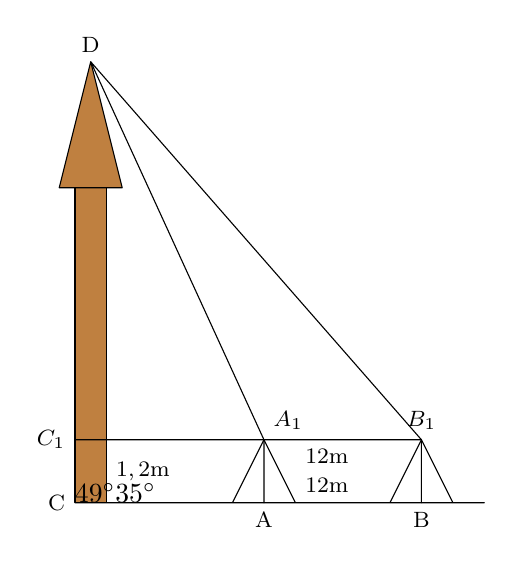
\begin{tikzpicture}[scale=0.8, font=\footnotesize, line join=round, line cap=round, >=stealth]
			\tkzDefPoints{0/0/C, 0/1/E, 3/1/M, 0.25/7/D, 5.5/1/N}
			\draw[fill=brown](0.5,0)--(0.5,5)--(0,5)--(0,0)--cycle;
			\draw(0,0)node[left]{C}--(6.5,0) (2.5,0)--(3,1)node[above right]{$A_1$}--(3.5,0) (5,0)--(5.5,1)--(6,0);
			\draw[fill=brown](5.5,1)node[above]{$B_1$}--(0,1) (0,5)--(-0.25,5)--(0.25,7)node[above]{D}--(0.75,5)--(0.5,5)--cycle;
			\draw(0,1)node[left]{$C_1$};
			\draw(3,0)node[below]{A} (5.5,0)node[below]{B} (0.5,0.5)node[right]{$1,2$m} (4,0)node[above]{$12$m} (4,1)node[below]{$12$m};
			\draw(3,0)--(3,1)--(0.25,7)--(5.5,1)--(5.5,0);
			\tkzMarkAngles[size=.7](D,M,E D,N,E)
			\tkzLabelAngles[pos=1,rotate=30](D,M,E){$49^\circ$}
			\tkzLabelAngles[pos=1,rotate=30](D,N,E){$35^\circ$}
	\end{tikzpicture}}
	\loigiai{
		Ta có $\widehat{A_1DB_1}=49^{\circ}-35^{\circ}=14^{\circ}$.\\
		Theo định lý hàm số sin ta có
		\[\dfrac{A_1D}{\sin 14^{\circ}}=\dfrac{A_1B_1}{\sin 35^{\circ}} \Rightarrow A_1D=\dfrac{12 \cdot \sin 14^{\circ}}{\sin 35^{\circ}} \approx 28,45.\]
		Xét tam giác $A_1C_1D$ vuông tại $C_1$. Khi đó  ta có $\sin 49^{\circ}=\dfrac{DC_1}{AD_1} \Rightarrow DC_1=28,45\sin 49^{\circ} \approx 21,47$. \\
		Vậy $CD=CC_1+C_1D=1,2+21,47=22,67$.
	}
\end{vd}

\subsection{BÀI TẬP TỰ LUYỆN}

\begin{baitap}
	Tam giác $ABC$ có $b=4\sqrt{3},c=4,\widehat{A}=30^{0}$. Tính $a$, $\widehat{B}$, $h_a$, $m_a$.
\end{baitap}

\begin{baitap}
	Tam giác $ABC$ có góc tù hay không nếu biết $a= 4$, $b= 5$, $c= 7$?
\end{baitap}

\begin{baitap}
	Giải tam giác $ABC$, biết
	\begin{tasks}(2)
		\task $a=b=6$; $\widehat{C}=54^{\circ}$
		\task $c=7$ ; $b=23\text{; }\widehat{A}=130^{\circ}$ 
		\task $c=14\text{; }\widehat{A}=60^{\circ}\text{; }\widehat{B}=40^{\circ}$
		\task $b=35\text{; }\widehat{A}=40^{\circ}\text{; }\widehat{C}=120^{\circ}$ 
		\task $a=14\text{; }b=18\text{; }c=20$ 
		\task $a=6\text{; }b=7,3\text{; }c=4,8$
	\end{tasks}
\end{baitap}

\begin{baitap}
	Tam giác $ABC$ có $a= 5$, $c= 5$ và $\cos B=\dfrac{3}{5}$. Tính $S$, $R$ và $r$
\end{baitap}

\begin{baitap}
	Cho tam giác $ABC$, có $AC= 13$, $AB+BC= 22$ và $\widehat{B}=60^{\circ}$. Tính độ dài các cạnh $AB$, $BC$ và diện tích tam giác $ABC$.
\end{baitap}

\begin{baitap}
	Cho $\Delta ABC$ có $\widehat{A}=90^\circ$, bán kính đường tròn ngoại tiếp $R=7$ và bán kính đường tròn nội tiếp là $r=3$. Tính diện tích $S$ của tam giác.
	\loigiai{
		Gọi $I$ là tâm đường tròn nội tiếp của $\Delta ABC$.
		\\ Gọi tiếp điểm của đường tròn nội tiếp $(I)$ với các cạnh $BC,CA, AB$ lần lượt là $D,E,F$.
		\\ Vì $\Delta ABC$ vuông tại A nên $BC=2R=14$ và $AE=AF=r=3$.
		\\ Ta có $p=\dfrac{AB+AC+BC}{2}=AE+BC=14+3=17$
		\\ Vậy $S=pr=17\cdot 3=51$}
\end{baitap}

\begin{baitap}%[0H2B3-3]
	Cho tam giác $ABC$. Chứng minh
	\begin{enumEX}{1}
		\item Góc $A$ nhọn $ \Leftrightarrow a^2<b^2+c^2$.
		\item Góc $A$ tù $ \Leftrightarrow a^2>b^2+c^2$.
		\item Góc $A$ vuông $ \Leftrightarrow a^2=b^2+c^2$.
	\end{enumEX}
	\loigiai{\begin{enumerate}
			\item Góc $A$ nhọn $\Leftrightarrow\cos A>0\Leftrightarrow\dfrac{b^2+c^2-a^2}{2bc}>0\Leftrightarrow a^2<b^2+c^2$.
			\item Góc $A$ tù $\Leftrightarrow\cos A<0\Leftrightarrow\dfrac{b^2+c^2-a^2}{2bc}<0\Leftrightarrow a^2>b^2+c^2$.
			\item Góc $A$ vuông $\Leftrightarrow\cos A=0\Leftrightarrow\dfrac{b^2+c^2-a^2}{2bc}=0\Leftrightarrow a^2=b^2+c^2$.
	\end{enumerate}}
\end{baitap}

\begin{baitap}%[0H2B3-2]
	Tam giác $ABC$ có $AB= c$; $BC=a$; $CA= b.$ Các cạnh $a$, $b$, $c$ liên hệ với nhau bởi đẳng thức $b(b^2 -a^2) = c(a^2 -c^2)$. Tính số đo góc $\widehat{BAC}$.
	\loigiai{
		Theo định lý hàm côsin, ta có $$\cos \widehat{BAC}= \dfrac{AB^2 + AC^2 - BC^2}{2 \cdot AB\cdot AC}= \dfrac{c^2 + b^2 -a^2}{2bc}.$$
		Mà 
		\begin{eqnarray*}
			& & b(b^2 -a^2) = c(a^2 -c^2) \\ 
			& \Leftrightarrow & b^3 -a^2 b = a^2 c -c^3 \\
			& \Leftrightarrow &-a^2 (b+c) + (b+c)(b^2 + c^2 -bc)=0\\
			& \Leftrightarrow & b^2 + c^2 - a^2 =bc.
		\end{eqnarray*} 
		Khi đó $\cos \widehat{BAC} = \dfrac{bc}{2bc}= \dfrac{1}{2}$.\\
		Vậy $\widehat{BAC}= 60^\circ$.
	}
\end{baitap}

\begin{baitap}%[0H2K3-2]
	Cho tam giác $ABC$. Chứng minh rằng điều kiện cần và đủ để hai trung tuyến kẻ từ $B$ và $C$ vuông góc với nhau là $b^2+c^2=5a^2$. 
	\loigiai{Gọi $G$ là trọng tâm của tam giác $ABC$.\\
		Khi đó hai trung tuyến kẻ từ $B$ và $C$ vuông góc với nhau khi và chỉ khi $\triangle GBC$ vuông tại $G$\\
		$\Leftrightarrow GB^2+GC^2=BC^2\Leftrightarrow\left(\dfrac{2}{3}m_b\right)^2+\left(\dfrac{2}{3}m_c\right)^2=a^2$.\qquad (*)\\
		Mặt khác theo công thức đường trung tuyến, ta có $m_b^2=\dfrac{2(a^2+c^2)-b^2}{4},m_c^2=\dfrac{2(a^2+b^2)-c^2}{4}$.\\
		Suy ra $\begin{aligned}[t]
			(*)\Leftrightarrow\,&\dfrac{4}{9}(m_b^2+m_c^2)=a^2\\
			\Leftrightarrow\,&\dfrac{4}{9}\left[\dfrac{2(a^2+c^2)-b^2}{4}+\dfrac{2(a^2+b^2)-c^2}{4}\right]=a^2\\
			\Leftrightarrow\,&4a^2+b^2+c^2=9a^2\,\Leftrightarrow\,b^2+c^2=5a^2.
		\end{aligned}$}
\end{baitap}

\begin{baitap}%[0H2B3-3]
	Cho tam giác $ABC$ thỏa mãn $\sin A=2\sin B\cdot\cos C$. Chứng minh $ABC$ là tam giác cân. 
	\loigiai{Ta có $\begin{aligned}[t]
			\sin A=2\sin B\cdot\cos C&\Leftrightarrow\dfrac{a}{2R}=2\cdot\dfrac{b}{2R}\cdot\dfrac{a^2+b^2-c^2}{2ab}\\
			&\Leftrightarrow a^2=a^2+b^2-c^2\Leftrightarrow b^2=c^2 \Leftrightarrow b=c.
		\end{aligned}$\\
		Vậy $ABC$ là tam giác cân tại $A$.}
\end{baitap}


\begin{baitap}%[0H2K3-3]
	Cho tam giác $ABC$ thoả mãn $\sin A=\dfrac{\sin B+\sin C}{\cos B+\cos C}$. Chứng minh rằng tam giác $ABC$ vuông. 
	\loigiai{Ta có 
		$\begin{aligned}[t]
			\sin A=\dfrac{\sin B+\sin C}{\cos B+\cos C} &\Leftrightarrow \sin A(\cos B+\cos C)=\sin B+\sin C\\
			&\Leftrightarrow \dfrac{a}{2R}\left(\dfrac{c^2+a^2-b^2}{2ca}+\dfrac{a^2+b^2-c^2}{2ab}\right)=\dfrac{b+c}{2R} \\
			&\Leftrightarrow b\left(c^2+a^2-b^2\right)+c\left(a^2+b^2-c^2\right)=2b^2c+2c^2b\\
			&\Leftrightarrow b^3+c^3+b^2c+bc^2-a^2b-a^2c=0\\
			&\Leftrightarrow (b+c)\left(b^2+c^2\right)-a^2(b+c)=0\Leftrightarrow b^2+c^2=a^2.
		\end{aligned}$\\
		Vậy tam giác $ABC$ vuông tại $A$.}
\end{baitap}

\begin{baitap}%[0H2B3-2] 
	Cho tam giác $ABC$ thỏa mãn $\sin^2A = \sin^2B + \sin^2 C$.  Chứng minh rằng tam giác $ABC$ vuông. 
	\loigiai{
		Từ định lí sin suy ra $\sin A = \dfrac{a}{2R}$, $\sin B = \dfrac{b}{2R}$, $\sin C = \dfrac{c}{2R}$. \\
		Khi đó 
		\[
		\sin^2A = \sin^2B + \sin^2 C \Leftrightarrow \left (\dfrac{a}{2R}\right )^2 = \left (\dfrac{b}{2R}\right )^2 +\left (\dfrac{c}{2R}\right )^2 \Leftrightarrow a^2=b^2+c^2.
		\]
		Vậy tam giác $ABC$ vuông tại $A$. 
	}
\end{baitap}
\begin{baitap}%[Phạm Tuấn]%[0H2B3-4]
	\immini{
		Để đo chiều rộng $AB$ của một khúc sông, người ta chọn điểm $C$.  Sau đó,  đo khoảng cách $BC$, các góc $B$ và $C$. Biết rằng $BC = 200$ m, $\widehat{B} = 107^\circ$,  $\widehat{C} = 28^\circ$. Tìm chiều rộng $AB$ của khúc sông đó (làm tròn đến chữ số thập phân thứ nhất).
	}
	{
		\begin{tikzpicture}[scale=1]
			\coordinate (X) at (1,1);
			\foreach \i in {0,...,6}
			\foreach \j  in {0,...,2}  
			\draw[blue] ($(X)+({\i+0.5},{0.6*(\j)+0.4})$)--($(X)+({\i+0.7},{0.6*(\j)+0.4})$);
			\coordinate [label=above left:$A$](A) at (3,3);
			\coordinate [label=below left:$B$](B) at (3,1);
			\coordinate [label=right:$C$](C) at (5,0.5);
			\draw (X)--(8,1) (8,3)--(1,3) (A)--(B)--(C)--(A);
			\foreach \i in {A,B,C} \draw[fill=black] (\i) circle(1.2pt);
		\end{tikzpicture}
	}
	\loigiai{
		Ta có $\widehat{A}= 180^\circ -  \widehat{B} -\widehat{C} =180^\circ- 107^\circ - 28^\circ=55^\circ$. \\
		Áp dụng định lí sin ta có 
		\[
		\dfrac{AB}{\sin C} = \dfrac{BC}{\sin A} \Rightarrow AB = \dfrac{BC\sin C}{\sin A}  = \dfrac{200\sin 28^{\circ}}{\sin 55^{\circ}} \approx 113{,}6\mathrm{~m}. 
		\]
	}
\end{baitap}


\begin{baitap}
	Một tàu cá xuất phát từ đảo $A$, chạy $50 \mathrm{~km}$ theo hướng $N 24^{\circ} \mathrm{E}$ đến đảo $B$ để lấy thêm ngư cụ, rồi chuyển hướng $N 36^{\circ} \mathrm{W}$ chạy tiếp $130 \mathrm{~km}$ đến ngư trường $C$.
	\begin{enumEX}[a)]{1}
		\item Tính khoảng cách từ vị trí xuất phát $A$ đến $C$ (làm tròn đến hàng đơn vị, theo đơn vị đo kilômét).
		\item Tìm hướng từ $A$ đến $C$ (làm tròn đến hàng đơn vị, theo đơn vị độ).
	\end{enumEX}
	\loigiai{
		\begin{enumEX}[a)]{1}
			\item Từ giả thiết suy ra $\widehat{A B C}=\left(90^{\circ}-24^{\circ}\right)+\left(90^{\circ}-36^{\circ}\right)=120^{\circ}$. Áp dụng định lí côsin cho tam giác $A B C$ ta được
			$$
			\begin{aligned}
				A C^{2} &=A B^{2}+B C^{2}-2 \cdot A B \cdot B C \cdot \cos \widehat{A B C} \\
				&=2500+16900-2 \cdot 50 \cdot 130 \cdot\left(-\frac{1}{2}\right)=25900 .
			\end{aligned}
			$$
			Suy ra $A C=10 \sqrt{259} \approx 161(\mathrm{~km})$.
			\item Áp dụng định lí sin cho tam giác $A B C$ ta được sin $\widehat{C A B}=\dfrac{B C}{A C} \cdot \sin \widehat{A B C} \approx 0,6993$. Suy ra $\widehat{C A B} \approx 44^{\circ}$ và do đó $A C$ chếnh về hướng tây một góc $44^{\circ}-24^{\circ}=20^{\circ}$ so với phương bắc.\\
			Vậy hướng từ $A$ tới $C$ là $N 20^{\circ} \mathrm{W}$.
		\end{enumEX}
		\begin{center}
			\begin{tikzpicture}[smooth,font=\footnotesize,scale=0.9,>=latex]
				\path
				(0,0) coordinate (A)
				(1,2) coordinate (B)
				($(B)!2!-120:(A)$) coordinate (C)
				(0,2) coordinate (A1)
				(1,4) coordinate (B1)
				%($(M)!0.4!(N)$)coordinate (K)
				% Vẽ hướng
				(-7,3) coordinate (E)
				(-10,3) coordinate (W)
				(-8.5,1.5) coordinate (S)
				(-8.5,4.5) coordinate (N)
				($(N)!0.5!(S)$)coordinate (O)
				($(O)!1!-24:(N)$) coordinate (N1)
				($(O)!1!36:(N)$) coordinate (N2)
				;
				\draw
				pic["\scriptsize$24^\circ$",angle radius=16mm]{angle = B--A--A1}
				pic[draw,angle radius=8mm]{angle = B--A--A1}
				pic["\scriptsize$36^\circ$",angle radius=16mm]{angle = B1--B--C}
				pic[draw,angle radius=8mm]{angle = B1--B--C};
				\draw[thick] (A)--(B)--(C)--cycle;
				\draw[dashed] (A)--(A1)--(B)--(B1);
				\draw[line width=1pt,blue,<->] (W)node[left]{\scriptsize$W$}--(E)node[right]{\scriptsize$E$};
				\draw[line width=1pt,blue,<->] (S)node[below]{\scriptsize$S$}--(N)node[above]{\scriptsize$N$};
				\draw[line width=1pt,blue,->] (O)--(N1)node[right]{\scriptsize$N24^\circ E$};
				\draw[line width=1pt,blue,->] (O)--(N2)node[left]{\scriptsize$N36^\circ W$};
				\foreach \x/\g in {A/-90,B/0,C/90} \draw [fill=cyan] (\x) circle (.15) + (\g:.45) node{$\x$};
				\path 
				(A)--(B) node[right,midway,scale=.8]{$50$ km }
				(B)--(C) node[right,midway,scale=.7]{$130$ km };
			\end{tikzpicture}
		\end{center}
	}
\end{baitap}

\begin{baitap}
	Một tàu du lịch xuất phát từ bãi biển Đồ Sơn (Hải Phòng), chạy theo hướng $N 80^{\circ} \mathrm{E}$ với vận tốc $20 \mathrm{~km} / \mathrm{h}$. Sau khi đỉ được 30 phút, tàu chuyển sang hướng $E 20^{\circ} S$ giữ nguyên vận tốc và chạy tiếp 36 phút nữa đến đảo Cát Bà. Hỏi khi đó tàu du lịch cách vị trí xuất phát bao nhiêu kilômet?
	\loigiai{
		Coi điểm xuất phát là $A$, điểm tàu chuyển hướng là $B$ và đich đến là $C$. Theo giả thiết
		$$\widehat{A B C}=180^{\circ}-\left(10^{\circ}+20^{\circ}\right)=150^{\circ}$$
		Do tàu chạy từ $A$ tới $B$ với vận tốc $20 \mathrm{~km} / \mathrm{h}$ trong 30 phút, nên
		$$
		A B=20 \cdot \frac{30}{60}=10(\mathrm{~km})
		$$
		Do tàu chạy từ $B$ đến $C$ với vận tốc $20 \mathrm{~km} / \mathrm{h}$ trong 36 phút, nên
		$$
		B C=20 \cdot \frac{36}{60}=12(\mathrm{~km}) .
		$$
		Áp dụng định lí côsin cho tam giác $A B C$ ta được
		$$
		A C^{2}=A B^{2}+B C^{2}-2 \cdot A B \cdot B C \cdot \cos \widehat{A B C}=10^{2}+12^{2}-2 \cdot 10 \cdot 12 \cdot\left(-\frac{\sqrt{3}}{2}\right) \approx 452 .
		$$
		Suy ra $A C \approx \sqrt{452} \approx 21(\mathrm{~km})$.
		\begin{center}
			\begin{tikzpicture}[smooth,font=\footnotesize,scale=0.9,>=latex]
				\path
				(0,4) coordinate (X)
				(5,4) coordinate (Y)
				($(X)!0.5!(Y)$)coordinate (B)
				($(B)!1.5!10:(X)$) coordinate (A)
				($(B)!1.8!-20:(Y)$) coordinate (C)
				% Vẽ hướng
				(-7,3) coordinate (E)
				(-10,3) coordinate (W)
				(-8.5,1.5) coordinate (S)
				(-8.5,4.5) coordinate (N)
				($(N)!0.5!(S)$)coordinate (O)
				($(O)!1!-80:(N)$) coordinate (N1)
				($(O)!1!-20:(E)$) coordinate (E1)
				;
				\draw
				pic["\scriptsize$10^\circ$",angle radius=23mm]{angle = X--B--A}
				pic[draw,double,angle radius=8mm]{angle = X--B--A}
				pic["\scriptsize$20^\circ$",angle radius=23mm]{angle = C--B--Y}
				pic[draw,angle radius=8mm]{angle = C--B--Y};
				\draw[thick] (A)--(B)--(C)--cycle;
				\draw[dashed] (X)--(Y);
				\draw[line width=1pt,blue,<->] (W)node[left]{\scriptsize$W$}--(E)node[right]{\scriptsize$E$};
				\draw[line width=1pt,blue,<->] (S)node[below]{\scriptsize$S$}--(N)node[above]{\scriptsize$N$};
				\draw[line width=1pt,blue,->] (O)--(N1)node[above]{\scriptsize$N80^\circ E$};
				\draw[line width=1pt,blue,->] (O)--(E1)node[below]{\scriptsize$E20^\circ S$};
				\foreach \x/\g in {A/-170,B/90,C/-10} \draw [fill=cyan] (\x) circle (.15) + (\g:.45) node{$\x$};
			\end{tikzpicture}
		\end{center}
	}
\end{baitap}

\begin{baitap}
	Một cây cổ thụ mọc thẳng đứng bên lề một con dốc có độ dốc $10^{\circ}$ so với phương nằm ngang. Từ một điểm dưới chân dốc, cách gốc cây 31 m người ta nhìn đỉnh ngọn cây dưới một góc $40^{\circ}$ so với phương nằm ngang. Hãy tính chiều cao của cây.
	\loigiai{
		\immini{\begin{itemize}
				\item [$\bullet$] Áp dụng định lí sin cho tam giác $ABC$.
				\item [$\bullet$] Chiều cao của cây là $h \approx 20,23(\mathrm{~m})$.
		\end{itemize}}{
			\begin{tikzpicture}[smooth,font=\footnotesize,scale=0.9,>=latex]
				\path
				(0,0) coordinate (A)
				(4,0) coordinate (X)
				(4,3) coordinate (C)
				(4,0.7) coordinate (B)
				;
				\draw
				pic["\tiny$10^\circ$",angle radius=26mm]{angle = X--A--B}
				pic[draw,angle radius=10mm]{angle = X--A--B}
				pic["\tiny$30^\circ$",angle radius=18mm]{angle = B--A--C}
				pic[draw,angle radius=8mm]{angle = B--A--C};
				\draw[thick] (A)--(B)--(C)--cycle;
				\draw[dashed] (A)--(X)--(B);
				\foreach \x/\g in {A/-90,B/0,C/90} \draw [fill=cyan] (\x) circle (.05) + (\g:.45) node{$\x$};
				\path 
				(A)--(X) node[below,midway,scale=.8]{$31$ km }
				;
			\end{tikzpicture}
		}
	}
\end{baitap}

\begin{baitap}%[Phạm Tuấn]%[0H2B3-4]
	\immini{
		Để đo chiều cao $CH$ của một  tháp truyền hình, người ta chọn hai điểm quan sát $A$, $B$ trên mặt đất (hình vẽ).  Biết $\widehat{CAH} =51^\circ$, $\widehat{CBH} =66^\circ$ và $AB=75 \mathrm{~m}$, tính chiều cao của tháp.
	}
	{
		\begin{tikzpicture}[scale=1, font=\footnotesize, line join=round, line cap=round,>=stealth]
			\path
			(1,0) coordinate (A)
			(2,0) coordinate (B)
			(4,3.5) coordinate (C)
			(4,0) coordinate (H)
			(3.75,0) coordinate (U)
			(4.25,0) coordinate (V)
			;
			\draw[thick] (U)--(C)--(V); 
			\draw (B)--(C)--(A)--(V) ;
			\draw[dashed] (C)--(H) ;  
			\draw  
			($(C)!{1}!(U)$)--($(C)!{0.9}!(V)$)
			--($(C)!{0.8}!(U)$)--($(C)!{0.7}!(V)$)
			--($(C)!{0.6}!(U)$)--($(C)!{0.5}!(V)$)
			--($(C)!{0.4}!(U)$)--($(C)!{0.3}!(V)$)
			--($(C)!{0.2}!(U)$)--($(C)!{0.1}!(V)$)
			;
			
			\tkzMarkAngle[arc=l, size=0.6,mark=0](H,A,C)
			\tkzLabelAngle[pos=1](H,A,C) {$51^{\circ}$}
			\tkzMarkAngle[arc=ll, size=0.6,mark=0](H,B,C)
			\tkzLabelAngle[pos=1](H,B,C) {$66^{\circ}$}
			\foreach \x/\g in {A/-90,B/-90,C/90,H/-90} 
			\fill[black] (\x) circle (1pt)+(\g:3mm) node {$\x$};
		\end{tikzpicture}
	}
	
	\loigiai{
		Ta có $\widehat{ACB}=\widehat{CBH} - \widehat{CAH}=  66^\circ -51^\circ= 15^\circ$. \\
		Áp dụng định lí sin ta có
		\[
		\dfrac{AB}{\sin \widehat{ACB}} = \dfrac{BC}{\sin \widehat{CAH} } \Rightarrow BC = \dfrac{AB\sin \widehat{CAH}}{\sin \widehat{ACB}}  = \dfrac{75\sin 51^\circ}{\sin 15^\circ}.
		\]
		Suy ra $CH =BC\sin \widehat{CBH} = \dfrac{75 \sin 51^\circ \sin 66^\circ}{\sin 15^\circ} \approx 205{,}7\mathrm{~m}.$
	}
\end{baitap}

\begin{baitap}%[Phạm Tuấn]%[0H2B3-4]
	\immini{
		Trên ngọn đồi có một cái tháp cao $120 \mathrm{~m}$. Đỉnh tháp $B$ và chân tháp $C$ nhìn điểm $A$ ở chân đồi dưới các góc tương ứng bằng $35^{\circ}$ và $60^{\circ}$ so với phương thẳng đứng. Xác định chiều cao $H A$ của ngọn đồi. (Làm tròn đến phần mười)
	}
	{
		\begin{tikzpicture}[scale=1, font=\footnotesize, line join=round, line cap=round, >=stealth]
			\path 
			(0,0) coordinate (X)
			(1.1,2) coordinate (Y)
			(2,2) coordinate (Z)
			(5,0) coordinate (A)
			(1.5,5) coordinate (B)
			(1.5,2) coordinate (C)
			(1.5,0) coordinate (K)
			(1.3,2) coordinate (U)
			(1.8,2) coordinate (V) 
			(5,2) coordinate (H);
			\draw  
			($(B)!{1}!(U)$)--($(B)!{0.9}!(V)$)
			--($(B)!{0.8}!(U)$)--($(B)!{0.7}!(V)$)
			--($(B)!{0.6}!(U)$)--($(B)!{0.5}!(V)$)
			--($(B)!{0.4}!(U)$)--($(B)!{0.3}!(V)$)
			--($(B)!{0.2}!(U)$)--($(B)!{0.1}!(V)$)
			;
			\draw[thick]  (X)--(A)--(Z)--(Y)--(X);
			\draw (A)--(B)  (U)--(B)--(V) (Y)--($(Y)!{1.2}!(H)$)  (X)--($(X)!{1.2}!(A)$);
			\draw[->] (A)--(H) ; 
			\draw ($(A)!0.5!(H)$) node[right]{$h$};
			\draw[dashed](B)--(K) (A)--(C);
			
			\tkzMarkAngle[arc=l, size=0.6,mark=0](K,C,A)
			\tkzLabelAngle[pos=0.9](K,C,A) {$60^{\circ}$}
			\tkzMarkAngle[arc=ll, size=0.7,mark=0](K,B,A)
			\tkzLabelAngle[pos=1.1](V,B,A) {$35^{\circ}$}
			\foreach \x/\g in{A/-90,B/90,C/-130,H/90}
			\fill[black](\x) ($(\x)+(\g:3mm)$)node{$\x$}; 
		\end{tikzpicture}
	}
	\loigiai{
		Ta có $\widehat{BAC} = 60^\circ - 35^\circ =25^\circ $;  $\widehat{ACH} = 90^\circ - 60^\circ =30^\circ $\\
		Áp dụng định lí sin ta có
		\[
		\dfrac{AC}{\sin \widehat{ABC}} = \dfrac{BC}{\sin \widehat{BAC}} \Rightarrow AC =  \dfrac{BC\sin \widehat{ABC}}{\sin \widehat{BAC}}
		= \dfrac{120\sin 35^\circ}{\sin 25^\circ}.
		\]
		Suy ra $AH =AC \sin \widehat{ACH} = \dfrac{120 \sin 35^\circ \sin 30^\circ }{\sin 25^\circ} \approx 81{,}4 \mathrm{~m}$.
	}
\end{baitap}

\begin{baitap}
	\immini{Một ô tô muốn đi từ địa điểm H đến địa điểm G, nhưng giữa H và G là một ngọn núi cao nên ô tô phải đi thành 2 đoạn từ H lên K (ô tô leo dốc lên núi) và từ K đến G (ô tô xuống núi). Các đoạn đường tạo thành tam giác $HKG$ với $HK = 15$ km, $KG = 20$ km và $\widehat{HKG}=120^\circ$. Giả sử cứ chạy $1$ km, ô tô tiêu thụ hết $0{,}3$ lít xăng. Giá thành xăng hiện nay là $13050$ đồng một lít xăng. Hỏi ô tô đi từ H đến G hết bao nhiêu tiền xăng?}
	{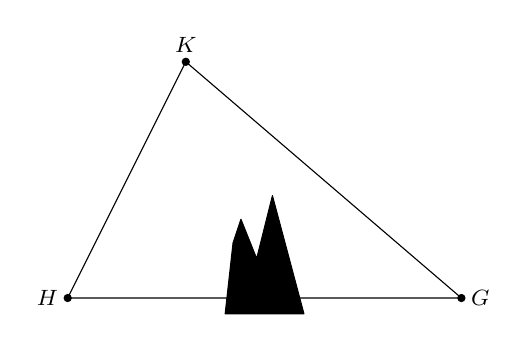
\begin{tikzpicture}[scale=1, font=\footnotesize, line join=round, line cap=round, >=stealth]
			\coordinate [label =left: $H$ ] (H) at (0,0);
			\coordinate [label =above: $K$ ] (K) at (1.5,3);
			\coordinate [label =right: $G$ ] (G) at (5,0);
			\draw (H)--(K)--(G)--cycle;	
			\draw[fill] (2,-0.2)--(2.1,0.7)--(2.2,1)--(2.4,0.5)--(2.6,1.3)--(3,-0.2)--cycle ;
			\foreach \diem in {H,K,G}\fill (\diem)circle(1.5pt);
		\end{tikzpicture}
	}
	\loigiai{Tổng quãng đường mà ô tô phải đi là$ S = HK + KG = 15 + 20 = 35$ km.\\	
		Ô tô đi hết quãng đường tiêu thụ hết số lít xăng là 	$35 \cdot 0{,}3 = 10{,}5$ lít.\\	
		Ô tô đi từ H đến G hết số tiền xăng là
		$10{,}5 \cdot 13050 = 137025$ đồng.}
\end{baitap}

\begin{baitap}%[0H2B3-4]
	\immini
	{
		Để đo khoảng cách từ vị trí $A$ đến vị trí $B$ ở hai bên bờ một cái ao, bạn An đi dọc bờ ao từ vị trí $A$ đến vị trí $C$ và tiến hành đo các góc $BAC$, $BCA$. Biết $AC=25 \text{ m}$, $\widehat{BAC}=59{,}95^\circ$, $\widehat{BCA}=82{,}15^\circ$ (hình vẽ bên). Hỏi khoảng cách từ vị trí $A$ đến vị trí $B$ là bao nhiêu mét (làm tròn kết quả đến hàng đơn vị)?
		}
	{
		\begin{tikzpicture}[scale=1,font=\footnotesize,line cap=round,line join=round,>=stealth]
			\def\a{3.75}
			\path (0:0) coordinate(A) (59.95:1) coordinate(a) (0:\a) coordinate(C)  + (97.85:1) coordinate(c)  (intersection of A--a and C--c) coordinate(B);
			\fill[cyan!60] (-.5,2) .. controls +(-70:2) and +(150:1) .. (2.5,1) .. controls +(-15:2) and +(-30:1) .. (4.5,3.5) .. controls +(150:1) and +(40:1) .. (2,4) .. controls +(-150:1.5) and +(100:2) .. cycle;
			\draw (A)--(B)--(C)--cycle;
			\foreach \d/\g in {A/-135, B/90, C/-45}
			\fill (\d) circle(1pt) node[shift={(\g:.3)}]{$\d$};
			\path (A)--(C) node[midway,below]{$25$ m} pic[draw,angle radius=.3cm]{angle=C--A--B} (A) node[shift={(20:.8)}]{$59{,}95^\circ$} pic[draw,angle radius=.3cm]{angle=B--C--A} pic[draw,angle radius=.35cm]{angle=B--C--A} (C) node[shift={(150:.7)}]{$82{,}15^\circ$};
			
		\end{tikzpicture}
	}
	\loigiai
	{
		Trong tam giác $ABC$ ta có
		\[\widehat{A}+\widehat{B}+\widehat{C}=180^\circ \Rightarrow \widehat{B}=180^\circ - \left(\widehat{A}+\widehat{C}\right) \Rightarrow \widehat{B} = 180^\circ - \left(59{,}95^\circ + 82{,}15^\circ\right) = 37{,}9^\circ.\]
		Áp dụng định lí sin trong tam giác $ABC$ ta có
		\[\dfrac{AB}{\sin C} = \dfrac{AC}{\sin B} \Rightarrow AB = \dfrac{AC\sin C}{\sin B} = \dfrac{25\sin 82{,}15^\circ}{\sin 59{,}95^\circ} \approx 29 \text{ m}.\]
		Vậy khoảng cách từ vị trí $A$ đến vị trí $B$ gần bằng $29$ mét.
	}
\end{baitap}

\begin{baitap}%[0H2B3-1] 
	\immini{
		Để đo bán kính của một chiếc đĩa cổ chỉ còn lại một phần, các nhà khảo cổ chọn $3$ điểm trên chiếc đĩa (hình vẽ) và tiến hành đo được kết quả như sau: $\widehat{A}=33^\circ$, $BC=15{,}3 \mathrm{~cm}$. Tính bán kính của chiếc đĩa (làm tròn kết quả đến hàng phần mười).
	}
	{
		\begin{tikzpicture}[scale=1, font=\footnotesize, line join=round, line cap=round,>=stealth]
			\coordinate (O) at (0,0); 
			\coordinate (A) at ($(O)+(131.4:3)$) ; 
			\coordinate (B) at ($(O)+(101.6:3)$) ; 
			\coordinate (C) at ($(O)+(41.7:3)$) ; 
			\coordinate (D) at ($(O)+(140:3)$) ; 
			\coordinate (E) at ($(O)+(90:1)$) ; 
			\coordinate (F) at ($(O)+(18:3)$) ; 
			\draw
			(D) 
			.. controls ++(0:0.5) and ++(150:0.5) .. (E)
			.. controls ++(180:-0.5) and ++(160: 0.5) .. (F)
			;
			\draw (A)--(B)--(C)--(A)  ; 
			\draw  (F) arc (18:140:3);
			\foreach \x/\g in {A/140,B/90,C/60} 
			\fill[black] (\x) circle (1.1pt)+(\g:3mm) node {$\x$};
		\end{tikzpicture}
	}
	\loigiai{
		Áp dụng định lí sin suy ra bán kính của chiếc đĩa là
		\[
		R = \dfrac{BC}{2\sin A} = \dfrac{15,3}{2\sin 33^\circ} \approx 13{,}8 \mathrm{~(cm)}. 
		\]
	}
\end{baitap}

\begin{baitap}%[0H2K3-4]
	\immini
	{
		Bạn $A$ đứng ở đỉnh của tòa nhà và quan sát chiếc diều, nhận thấy góc nâng (góc nghiêng giữa phương từ mắt của bạn $A$ tới chiếc diều và phương nằm ngang) là $\alpha=35^\circ$; khoảng cách từ đỉnh tòa nhà tới mắt bạn $A$ là $1{,}5 \text{ m}$. Cùng lúc đó ở dưới chân tòa nhà, bạn $B$ cũng quan sát chiếc diều và thấy góc nâng là $\beta=75^\circ$; khoảng cách từ mặt đất tới mắt bạn $B$ cũng là $1{,}5 \text{ m}$. Biết chiều cao của tòa nhà là $h=20\text{ m}$ (minh họa ở hình bên). Chiếc diều bay cao bao nhiêu mét so với mặt đất (làm tròn kết quả đến hàng đơn vị)?
		}
	{
		\begin{tikzpicture}[scale=.8,font=\footnotesize,line cap=round,line join=round,>=stealth]
			\draw (0,0) coordinate(O)grid (2,6);
			\draw (2,6)--(2,6.5) coordinate(A) (2,.5) coordinate(B);
			\path[shift={(B)}] (75:1) coordinate(b);
			\path[shift={(A)}] (35:1) coordinate(a);
			\path (intersection of A--a and B--b) coordinate(C) ($(A)!.8!(C)$) coordinate(D) ($(O)!(C)!(5,0)$) coordinate(H) ($(C)!(A)!(H)$) coordinate(I) ($(C)!(B)!(H)$) coordinate(J);
			\path[shift={(C)}] (65:.4) coordinate(E) (140:1) coordinate(F) ($(C)!.6!(F)$) coordinate(G);
			\fill[cyan!80] (C)--(D) .. controls + (130:.5) and +(-100:.3) .. (F) .. controls +(10:.3) and +(120:.4) ..(E) .. controls +(-120:.3) and +(70:.2) .. cycle;
			\fill[blue!80!black] (C)--(G) .. controls +(50:.3) and +(130:.2) .. (E) .. controls +(-120:.3) and +(70:.2) .. cycle;
			\fill[blue!80!black] (D) .. controls + (130:.5) and +(-100:.3) .. (F) -- (G) .. controls +(-130:.3) and +(110:.2) .. cycle;
			\draw[color=blue!80!red] (C) .. controls +(-10:.6) and +(150:.5) .. (5,7);
			\draw[color=blue!80!red] (C) .. controls +(-15:.6) and +(150:.5) .. (4.8,6.9);
			\draw (A)--(C)--(B) (2,0)--(H);
			\draw[dashed] (C)--(H) (A)--(I) (B)--(J);
			\path (O)--(0,6) node[midway,left]{$h$} (A) node[shift={(180:.3)}]{$A$} (B) node[shift={(-45:.3)}]{$B$};
			\begin{scope}
				\clip (C)--(A)--(I);
				\draw (A) circle(.4) node[shift={(15:.5)}]{$\alpha$};
			\end{scope}
			\begin{scope}
				\clip (C)--(B)--(J);
				\draw[double] (B) circle(.4) node[shift={(35:.55)}]{$\beta$};
			\end{scope}
			
		\end{tikzpicture}
	}
	\loigiai
	{
		\immini
		{
			Kí hiệu $C$ là vị trí của chiếc diều.\\
			Từ điểm $B$ vẽ đường thẳng $Bx$ vuông góc với $AB$.\\
			Từ điểm $C$ kẻ $CH\perp Bx$ ($H$ thuộc $Bx$).\\
			Từ điểm $A$ kẻ $AK\perp CH$ ($K$ thuộc $CH$).\\
			Khi đó $\widehat{CAK}=\alpha$ và $\widehat{CBH}=\beta$.\\
			Chiều cao của diều so với mặt đất chính là độ dài đoạn thẳng $CH$.\\
			Vì khoảng cách từ đỉnh tòa nhà tới mắt bạn $A$ và khoảng cách từ mặt đất tới mắt bạn $B$ đều là $1{,}5 \text{ m}$ nên $AB=h=20\text{ m}$.\\
			Tứ giác $ABHK$ là hình chữ nhật.\\
			$\widehat{CAB} = \widehat{CAK}+\widehat{KAB} = 35^\circ + 90^\circ = 125^\circ$.\\
			$\widehat{CBA} = \widehat{ABH}-\widehat{CBH} = 90^\circ-75^\circ = 15^\circ$.\\
			Trong tam giác $ABC$ ta có
			\[\widehat{C} = 180^\circ - \left(\widehat{A}+\widehat{B}\right) = 180^\circ - \left(125^\circ+15^\circ\right) = 40^\circ.\]
		}
		{
			\begin{tikzpicture}[scale=.8,font=\footnotesize,line cap=round,line join=round,>=stealth]
				\path (0,0) coordinate(B) (0,6) coordinate(A) + (35:1) coordinate(a) (75:1) coordinate(b) (intersection of A--a and B--b) coordinate(C) ($(B)!(C)!(1,0)$) coordinate(H) ($(C)!(A)!(H)$) coordinate(K);
				\draw (A)--(B)--(C)--cycle (C)--(H)--(B) (A)--(K);
				\foreach \d/\g in {A/180, B/-135, C/45, H/-45, K/0}
				\fill (\d) circle(1pt) node[shift={(\g:.3)}]{$\d$};
				\path pic[draw,angle radius=.15cm]{right angle=A--K--C} pic[draw,angle radius=.15cm]{right angle=B--H--C};
				\begin{scope}
					\clip (C)--(A)--(I);
					\draw (A) circle(.4) node[shift={(15:.5)}]{$\alpha$};
				\end{scope}
				\begin{scope}
					\clip (C)--(B)--(J);
					\draw[double] (B) circle(.4) node[shift={(35:.55)}]{$\beta$};
				\end{scope}
				
			\end{tikzpicture}
		}
		\noindent
		Áp dụng định lí sin trong tam giác $ABC$ ta có
		\[\dfrac{AB}{ \sin C} = \dfrac{BC}{\sin A} \Rightarrow BC = \dfrac{AB\sin A}{\sin C} = \dfrac{20\sin 125^\circ}{\sin 40^\circ} \approx 25{,}49.\]
		Trong tam giác $CBH$ vuông tại $H$ ta có
		\[CH=BC\sin B \approx 25{,}49\sin 75^\circ \approx 24{,}6.\]
		Vậy chiếc diều bay cao khoảng $24{,}6$ mét so với mặt đất.
	}
\end{baitap}
